\chapter{آواشناسی آکوستیکی: موج صوتی، طیف، اسپکتروگرام و مدل منبع--فیلتر}

\section{توضیحات کلاس دربارهٔ ارزشیابی}

\begin{exambox}{نحوهٔ نمره‌دهی درس}
نمرهٔ درس: \textbf{۱۰ نمرهٔ عملی} (فعالیت‌ها و تمرین‌ها؛ احتمالاً گزارش یا «ارائه») و \textbf{۱۰ نمرهٔ نظری} (میان‌ترم و پایان‌ترم). سؤالات نظری از مطالب مطرح‌شده در کلاس طرح می‌شود. همچنین \textbf{تمرین اول دربارهٔ اسپکتروگرام است}؛ پس مفاهیم این فصل برای تمرین هم لازم است.
\end{exambox}

\section{مرور جلسهٔ قبل و طرح مسئله}

در جلسهٔ قبل با \term{آواشناسی تولیدی}{Articulatory Phonetics} آشنا شدیم: \term{نقشهٔ واکه‌ها}{Vowel Chart}، \term{محل تولید}{Place of Articulation} و \term{شیوهٔ تولید}{Manner of Articulation}. این مفاهیم رویدادهای داخل دهان را توصیف می‌کنند، اما پرسش اصلی این جلسه این است: \textbf{این ویژگی‌های تولیدی در موج فیزیکی صدا چه اثری می‌گذارند؟} هدف، یافتن یک \term{نگاشت}{Mapping} میان ویژگی‌های تولیدی (محل زبان، بازشدن دهان) و ویژگی‌های فیزیکی موج (فرکانس، دامنه، ساختار طیفی) است؛ نگاشتی که برای \eng{Speech-to-Text}، \eng{Text-to-Speech} و سایر سامانه‌های گفتاری مهم است.

\term{آواشناسی آکوستیکی}{Acoustic Phonetics} به بررسی خصوصیات فیزیکی موج صوتی گفتار می‌پردازد؛ در این فصل می‌بینیم رویدادهای تارهای صوتی و مجرای صوتی چگونه در این موج منعکس می‌شوند.

\section{موج صوتی، فرکانس پایه و زیر و بمی}

\term{شکل موج}{Waveform} نمایش سیگنال در \textbf{حوزهٔ زمان} است: محور افقی زمان و محور عمودی دامنه، یعنی انحراف فشار هوا از فشار محیط. صدای قوی‌تر یعنی اختلاف فشار بیشتر و قله‌های بلندتر.

\term{فرکانس}{Frequency} یعنی تعداد تکرار یک الگوی نوسانی در واحد زمان: اگر در $T$ ثانیه دقیقاً $N$ چرخهٔ کامل داشته باشیم، $f=N/T$ (هرتز). برای یک موج متناوب با \term{دوره تناوب}{Period} $T_0$ (مدت یک چرخه):
\[
F_0=\frac{1}{T_0},\qquad T_0=\frac{1}{F_0}.
\]
مثال: فاصلهٔ $10$ میلی‌ثانیه میان دو تکرار $\Rightarrow F_0=100$ هرتز (صدای مردانهٔ معمولی)؛ فاصلهٔ $5$ میلی‌ثانیه $\Rightarrow F_0=200$ هرتز (صدای زنانهٔ معمولی).

\boardfigure{0.7}{ch03-board-waveform-iy.png}{شکل موج واکهٔ \eng{[iy]}. الگوی تکرارشوندهٔ قله‌ها و درّه‌ها دیده می‌شود؛ مدت یک تکرار کامل، تناوب موج است.}

\begin{correctionbox}{شمردن قله‌ها همیشه $F_0$ را نمی‌دهد}
در موج پیچیدهٔ گفتار در هر دوره چند قلهٔ کوچک و بزرگ هست (اثر فرمنت‌ها)؛ آنچه باید اندازه گرفت مدت تکرار \emph{کل الگو} است، نه تعداد همهٔ قله‌ها. در عمل $F_0$ را روی فریم‌های کوتاه با الگوریتم‌هایی مانند خودهمبستگی (\eng{autocorrelation}) تخمین می‌زنند.
\end{correctionbox}

\begin{definitionbox}{فرکانس پایه و \eng{Pitch}}
موج حاصل از ارتعاش تارهای صوتی یک \term{فرکانس پایه}{Fundamental Frequency} ($F_0$) دارد که با ادراک \term{زیر و بمی}{Pitch} مرتبط است: $F_0$ بالاتر $\leftarrow$ صدای زیرتر؛ $F_0$ پایین‌تر $\leftarrow$ صدای بم‌تر.
\end{definitionbox}

\begin{correctionbox}{$F_0$ ویژگی فیزیکی است و \eng{Pitch} ویژگی ادراکی}
$F_0$ را از سیگنال اندازه می‌گیریم (هرتز) ولی \eng{Pitch} آن چیزی است که شنونده می‌شنود. رابطهٔ این دو یکنوا است اما خطی نیست (دو برابرشدن $F_0$ یعنی یک اکتاو بالاتر).
\end{correctionbox}

\textbf{چرا $F_0$ افراد متفاوت است؟} در توضیح ساده‌شدهٔ کلاس، تارهای ضخیم‌تر کندتر و تارهای نازک‌تر سریع‌تر می‌لرزند (حدود ۱۰۰ هرتز برای صدای مردانه و ۲۰۰ هرتز برای زنانه؛ اعداد تقریبی‌اند).
\begin{correctionbox}{دقیق‌تر: طول، جرم و کشش}
$F_0$ به \emph{طول، جرم و کشش} تارهای صوتی (و فشار هوای زیر چاکنای) بستگی دارد، نه فقط «ضخامت». تارهای مردان بالغ بلندتر و پرجرم‌ترند؛ گوینده نیز با تغییر کشش ماهیچه‌های حنجره می‌تواند $F_0$ خود را ارادی تغییر دهد.
\end{correctionbox}

\textbf{آیا \eng{Pitch} جنسیت را مشخص می‌کند؟} خیر. استاد از دانشجویان خواستند «آ» را یک بار عادی و بار دیگر بم‌تر یا زیرتر بگویند: با ثابت‌ماندن شکل دهان، فقط ارتعاش تارها عوض می‌شود. برخی زنان صدای بم و برخی مردان صدای زیر دارند. علاوه بر $F_0$، \term{طول مجرای صوتی}{Vocal Tract Length} هم مؤثر است (مجرای بلندتر، فرمنت‌های پایین‌تر)؛ پس برای مقایسهٔ گویندگان نباید به $F_0$ اکتفا کرد.

\section{تحلیل فرکانسی و تبدیل فوریه}

موج گفتار فقط یک فرکانس ندارد؛ ترکیبی از مؤلفه‌های فرکانسی است. برای دانستن اینکه \emph{چه فرکانس‌هایی} هست و \emph{هرکدام چه سهمی} دارد، از \term{تبدیل فوریه}{Fourier Transform} استفاده می‌کنیم. ایده: هر سیگنال را می‌توان مجموع چند موج سینوسی با فرکانس، دامنه و فاز مناسب دانست.

\boardfigure{0.7}{ch03-board-sum-sines.png}{جمع چند سینوسی با فرکانس‌های متفاوت یک موج پیچیده می‌سازد. تبدیل فوریه مسئلهٔ معکوس را حل می‌کند: از موج پیچیده، سینوسی‌های سازنده را پیدا می‌کند.}

\textbf{شهود ضرب داخلی.} استاد شباهت سیگنال با یک موج مبنا را با \term{ضرب داخلی}{Dot Product} سنجیدند: صفر یعنی آن مؤلفه سهمی ندارد؛ غیرصفر یعنی سهم دارد و علامت منفی یعنی فاز معکوس (شکل \ref{fig:ch03-dot-example}).

\begin{figure}[htbp]
\centering
\begin{tikzpicture}[rtl]
\node[draw=red!70!black, thick, rounded corners=6pt, inner sep=6pt, fill=softred] (x) {$x=(-1,\;\;1,\;\;-1,\;\;1)$};
\node[below=6mm of x, inner sep=0pt] (tab) {%
\renewcommand{\arraystretch}{1.5}%
\begin{tabular}{@{}lll@{}}
\toprule
\textbf{بردار مبنا} & \textbf{ضرب داخلی با $x$} & \textbf{نتیجه}\\
\midrule
$b_1=(\phantom{-}1,\;\phantom{-}1,\;\phantom{-}1,\;\phantom{-}1)$ & \lr{$-1+1-1+1=0$} & سهمی ندارد\\
$b_2=(-1,\,-1,\;\phantom{-}1,\;\phantom{-}1)$ & \lr{$1-1-1+1=0$} & سهمی ندارد\\
$b_3=(\phantom{-}1,\,-1,\;\phantom{-}1,\,-1)$ & \lr{$-1-1-1-1=-4$} & سهم کامل (فاز معکوس) \checkmark\\
\bottomrule
\end{tabular}};
\draw[red!70!black, thick, -{Stealth[length=2.2mm]}] (x) -- (tab.north);
\end{tikzpicture}
\caption{محاسبهٔ تخته: سیگنال $x$ (درون بیضی) با سه بردار مبنا مقایسه می‌شود؛ ضرب داخلی با دو بردار اول صفر و با بردار سوم $-4$ است (بازسازی‌شده از تختهٔ کلاس).}
\label{fig:ch03-dot-example}
\end{figure}

در عمل هر فریم کوتاه، رشته‌ای از $N$ نمونهٔ دامنه است و برای هر فرکانس شباهت آن با موج مبنای $e^{-j2\pi kn/N}$ سنجیده می‌شود:
\[
X[k]=\sum_{n=0}^{N-1}x[n]\,e^{-j2\pi kn/N}.
\]
خروجی برای هر فرکانس یک عدد مختلط $a+jb$ است؛ اندازهٔ آن \term{بزرگی}{Magnitude} $\sqrt{a^2+b^2}$ (سهم آن فرکانس) و زاویهٔ آن \term{فاز}{Phase} است.

\begin{correctionbox}{دو نکته دربارهٔ توضیح تخته}
(۱) ۵۱۲ در مثال تخته «تعداد نمونه‌های یک فریم» ($N=512$) است، نه نرخ نمونه‌برداری. (۲) «کندترین موج = \eng{Pitch}» دقیق نیست: کندترین موج مبنا فرکانس $f_s/N$ دارد و فقط فاصلهٔ نقاط شبکهٔ فرکانسی را تعیین می‌کند؛ در یک سیگنال متناوب، کندترین مؤلفهٔ \emph{واقعاً موجود} همان $F_0$ است.
\end{correctionbox}

نمونه‌ها: سیگنال $x(t)=A\sin(2\pi f t)$ در طیف یک‌طرفه تنها یک مؤلفه در $f$ دارد (مانند بوق ممتد)؛ ساختار آن بسیار ساده‌تر از گفتار است.

\section{هارمونیک‌ها}

\begin{definitionbox}{هارمونیک}
در یک صدای متناوب با فرکانس پایه $F_0$، مؤلفه‌های طیف در مضارب صحیح $F_0$ قرار می‌گیرند:
\[
F_n=n\,F_0,\qquad n=1,2,3,\dots
\]
هارمونیک اول همان فرکانس پایه است ($H_1=F_0$)، $H_2=2F_0$ و ... . دامنهٔ هر هارمونیک می‌تواند متفاوت باشد.
\end{definitionbox}

مثال: برای $F_0=100$ هرتز، هارمونیک‌های اول تا پنجم در $100,200,300,400,500$ هرتز هستند.

\begin{figure}[htbp]
\centering
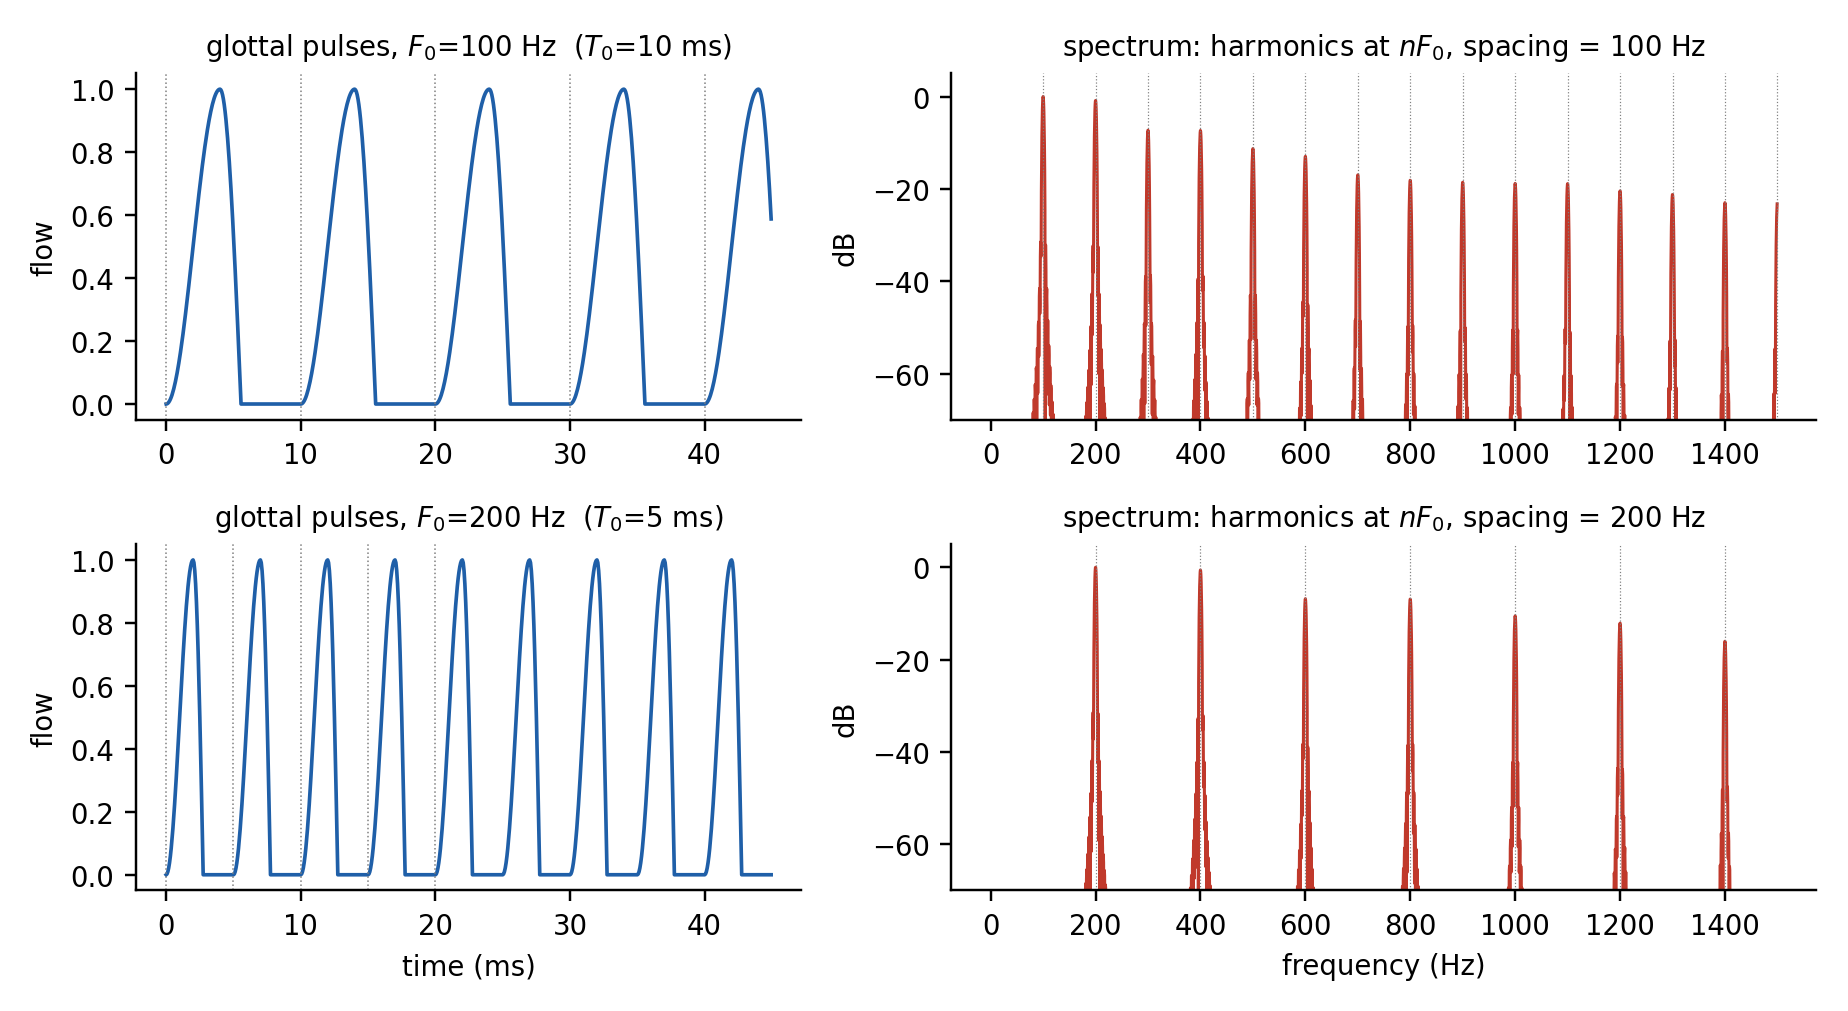
\includegraphics[width=0.95\textwidth]{../assets/figures/ch03-glottal-harmonics.png}
\caption{بالا: دنبالهٔ تپ‌های ساده‌شدهٔ هوای چاکنای با $F_0=100$ هرتز و طیف آن. پایین: همان با $F_0=200$ هرتز. هارمونیک‌ها در مضارب صحیح $F_0$ ظاهر می‌شوند و فاصلهٔ آن‌ها دقیقاً $F_0$ است (شکل افزوده).}
\end{figure}

فاصلهٔ دو هارمونیک متوالی برابر $F_0$ است؛ پس هرچه $F_0$ بزرگ‌تر (صدای زیرتر)، هارمونیک‌ها دورتر از هم‌اند و هرچه کوچک‌تر (صدای بم‌تر)، فشرده‌ترند. به همین دلیل از فاصلهٔ خطوط هارمونیکی در اسپکتروگرام می‌توان $F_0$ و تغییرات آن را خواند. اما $F_0$ و هارمونیک‌ها فقط «منبع» را توصیف می‌کنند و نمی‌گویند چرا «آ» با «ای» فرق دارد.

\section{اسپکتروگرام}

تبدیل فوریهٔ کل گفتار یک طیف واحد می‌دهد و زمان را از دست می‌دهد، در حالی که گفتار ایستا نیست. \term{اسپکتروگرام}{Spectrogram} تغییرات محتوای فرکانسی را در طول زمان نمایش می‌دهد. مراحل ساخت (\term{تبدیل فوریهٔ زمان-کوتاه}{Short-Time Fourier Transform, STFT}):
\begin{enumerate}
  \item سیگنال به پنجره‌ها یا فریم‌های کوتاه (مثلاً ۲۵ میلی‌ثانیه) بریده می‌شود (\eng{Windowing})؛ پنجره‌ها می‌توانند هم‌پوشانی (\eng{Overlap}) داشته باشند یا نداشته باشند؛
  \item روی هر فریم تبدیل فوریه اعمال و بزرگی طیف به دست می‌آید؛
  \item طیف‌ها به‌ترتیب زمان کنار هم چیده می‌شوند.
\end{enumerate}

محور افقی زمان، محور عمودی فرکانس و رنگ یا روشنایی هر نقطه، بزرگی (انرژی) آن مؤلفه در آن لحظه است. رنگ گرم یعنی بزرگی بالا، که معمولاً هارمونیک صدای ورودی است.

\boardfigure{0.7}{ch03-board-spectrogram-harmonics.png}{اسپکتروگرام یک صدای تقریباً پایدار: رنگ گرم یعنی بزرگی بالا (شباهت زیاد آن فرکانس با سیگنال ورودی، معمولاً هارمونیک)، رنگ سرد یعنی بزرگی پایین. خطوط افقی پررنگ هارمونیک‌ها هستند.}

\begin{correctionbox}{مقیاس رنگ معمولاً دسی‌بل است}
رنگ معمولاً لگاریتم بزرگی ($20\log_{10}|X|$) را نشان می‌دهد، نه خود بزرگی؛ و فاز کنار گذاشته می‌شود.
\end{correctionbox}

\begin{warningbox}{فرکانس و دامنه دو چیز متفاوت‌اند}
فرکانس یعنی سرعت نوسان و دامنه یعنی اندازهٔ نوسان. قرار داشتن یک مؤلفه در فرکانس بالاتر به معنی دامنهٔ بیشتر نیست. این تمایز در کلاس چند بار تأکید شد: در اسپکتروگرام «ارتفاع» فرکانس است و «پررنگی» دامنه.
\end{warningbox}

\section{مدل منبع--فیلتر}

وقتی فردی از «آ» به «ای» می‌رود و $F_0$ را ثابت نگه می‌دارد، صدا فرق می‌کند؛ این تغییر از $F_0$ نمی‌آید. پس مدل کامل‌تری لازم است.

\begin{definitionbox}{مدل منبع--فیلتر (\lr{Source--Filter})}
تولید گفتار به دو بخش (در تقریب مدل، مستقل) تقسیم می‌شود:
\begin{itemize}
  \item \textbf{منبع (\lr{Source}):} برای صداهای واک‌دار، ارتعاش تارهای صوتی که موجی دوره‌ای با $F_0$ و هارمونیک‌هایش تولید می‌کند؛
  \item \textbf{فیلتر (\lr{Filter}):} مجرای صوتی (\eng{Vocal Tract}) که بسته به شکلش بخش‌هایی از طیف را تقویت (تشدید) و بخش‌هایی را تضعیف می‌کند.
\end{itemize}
\end{definitionbox}

در حوزهٔ فرکانس، خروجی حاصل‌ضرب طیف منبع در پاسخ فرکانسی فیلتر است (در حوزهٔ زمان، کانولوشن؛ و در مقیاس لگاریتمی، جمع):
\[
\text{\lr{Output}}(f)=\text{\lr{Source}}(f)\times\text{\lr{Filter}}(f).
\]

\begin{figure}[htbp]
\centering
\begin{tikzpicture}[rtl, node distance=1.2cm, every node/.style={font=\small},
  box/.style={draw, rounded corners, minimum width=2.8cm, minimum height=1.1cm, align=center},
  arr/.style={-{Stealth[length=2.5mm]}, thick}]
  \node[box, fill=blue!10] (src) {منبع\\ \lr{Source}\\ \footnotesize تارهای صوتی};
  \node[box, left=of src, fill=green!10] (fil) {فیلتر\\ \lr{Filter}\\ \footnotesize مجرای صوتی};
  \node[box, left=of fil, fill=orange!12] (out) {خروجی\\ \lr{Output}\\ \footnotesize موج گفتار};
  \draw[arr] (src) -- (fil); \draw[arr] (fil) -- (out);
  \node[below=0.5mm of src, font=\scriptsize, align=center] {\lr{$F_0$ and harmonics}};
  \node[below=0.5mm of fil, font=\scriptsize, align=center] {\lr{formants $F_1,F_2,F_3$}};
  \node[below=0.5mm of out, font=\scriptsize, align=center] {\lr{harmonics shaped by formants}};
\end{tikzpicture}
\caption{نمای ساده‌شدهٔ مدل منبع--فیلتر برای صداهای واک‌دار (شکل افزوده).}
\end{figure}

استاد مجرا را شبیه یک لوله در نظر گرفتند: هر تغییر در موقعیت زبان، باز بودن دهان، فک، لب‌ها و محل تنگ‌شدگی، مشخصات فیلتر را عوض می‌کند. این همان پیوند مطلوب ماست: تغییر وضعیت اندام‌ها $\leftarrow$ تغییر قابل مشاهده در طیف موج.

\begin{figure}[htbp]
\centering
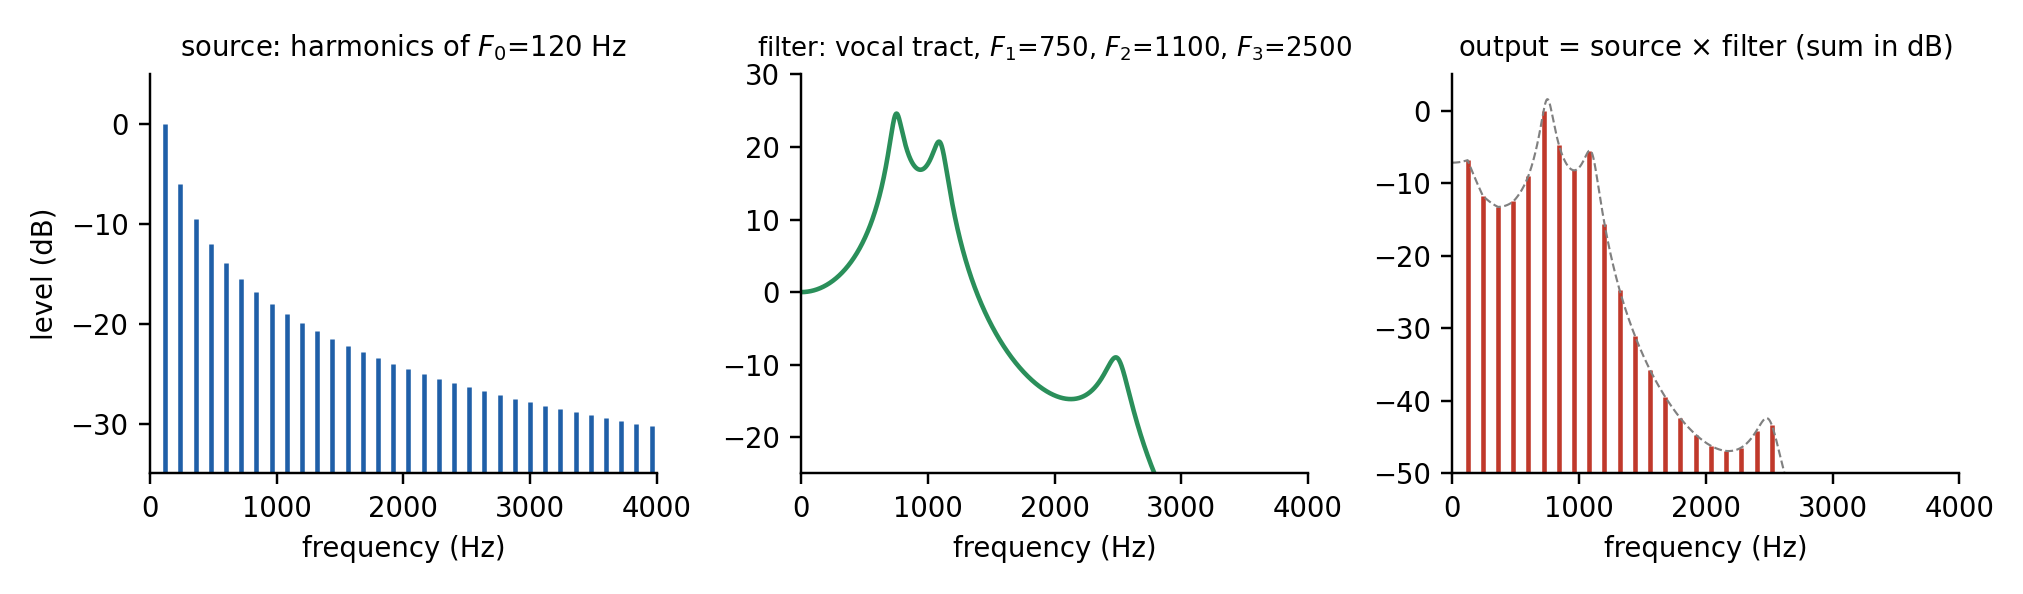
\includegraphics[width=0.95\textwidth]{../assets/figures/ch03-source-filter-spectra.png}
\caption{نمونهٔ عددی با $F_0=120$ هرتز: (الف) هارمونیک‌های منبع؛ (ب) پاسخ فرکانسی مجرا با فرمنت‌های $F_1=750$، $F_2=1100$ و $F_3=2500$ هرتز؛ (ج) خروجی (جمع دو منحنی در مقیاس دسی‌بل). خط‌چین پوش طیفی است (شکل افزوده).}
\end{figure}

\begin{correctionbox}{استقلال منبع و فیلتر تقریبی است}
مدل فرض می‌کند تغییر $F_0$ فرمنت‌ها را جابه‌جا نمی‌کند و برعکس؛ این تقریب برای بیشتر تحلیل‌ها خوب است، ولی برهم‌کنش منبع و مجرا و تابش از لب‌ها را نادیده می‌گیرد.
\end{correctionbox}

\textbf{آیا همهٔ صداها از تارهای صوتی می‌آیند؟} خیر؛ همخوان‌های بی‌واک مانند «س» منبعی از نویز آشفتگی جریان هوا دارند و هارمونیک ندارند. مدل «منبع = ارتعاش تارها» فقط برای صداهای واک‌دار است و تمرکز این جلسه بر همین حالت بود.

\section{فرمنت‌ها}

\begin{definitionbox}{فرمنت (\lr{Formant})}
فرمنت‌ها نواحی تشدید مجرای صوتی‌اند؛ نواحی فرکانسی که فیلتر آن‌ها را تقویت می‌کند. در طیف، قله‌ای پهن در پوش طیف و در اسپکتروگرام، نواری پررنگ‌اند. فرمنت‌ها بر اساس ترتیب فرکانسی نام‌گذاری می‌شوند: $F_1<F_2<F_3<\cdots$ (نه ترتیب زمانی).
\end{definitionbox}

فرمنت یک هارمونیک منفرد نیست؛ یک \emph{ناحیه} است که دامنهٔ چند هارمونیک مجاور را بالا می‌برد. فرمنت‌ها متعلق به فیلترند و ما هنگام تحلیل آن‌ها را \emph{نمی‌سازیم}، بلکه از سیگنال شناسایی می‌کنیم.

\textbf{ارتباط با نقشهٔ واکه‌ها} (مهم‌ترین ارتباط جلسه):
\begin{center}
\begin{tabular}{ll}
\toprule
ویژگی تولیدی & ویژگی آکوستیکی \\
\midrule
ارتفاع زبان / میزان بازشدگی دهان & $F_1$ \\
جلو یا عقب بودن زبان & $F_2$ \\
\bottomrule
\end{tabular}
\end{center}
\begin{itemize}
  \item $F_1$ برای واکه‌های بازتر بالاتر است: «آ» $F_1$ بالاتری از «ای» دارد.
  \item $F_2$ برای واکه‌های جلویی بالاتر و برای عقبی پایین‌تر است.
\end{itemize}

\boardfigure{0.8}{ch03-board-formants-iau.png}{اسپکتروگرام سه واکهٔ \eng{/i/}، \eng{/a/} و \eng{/u/} با خطوط افقی موقعیت $F_1$ تا $F_3$. در \eng{/i/} فاصلهٔ $F_1$ و $F_2$ بسیار زیاد است؛ در \eng{/a/} فرمنت اول بالاتر است؛ در \eng{/u/} هر دو فرمنت اول و دوم پایین‌اند.}

\begin{addedbox}{مقادیر نوعی فرمنت (مردان بالغ، تقریبی)}
\begin{center}
\begin{tabular}{lccc}
\toprule
واکه & $F_1$ & $F_2$ & $F_3$ \\
\midrule
\eng{/i/} («ای») & $270$ & $2290$ & $3010$ \\
\eng{/a/} («آ») & $730$ & $1090$ & $2440$ \\
\eng{/u/} («او») & $300$ & $870$ & $2240$ \\
\bottomrule
\end{tabular}
\end{center}
میانگین‌های واکه‌های انگلیسی (پترسون و بارنی، ۱۹۵۲) برحسب هرتز؛ فقط برای نشان‌دادن الگو.
\end{addedbox}

\begin{figure}[htbp]
\centering
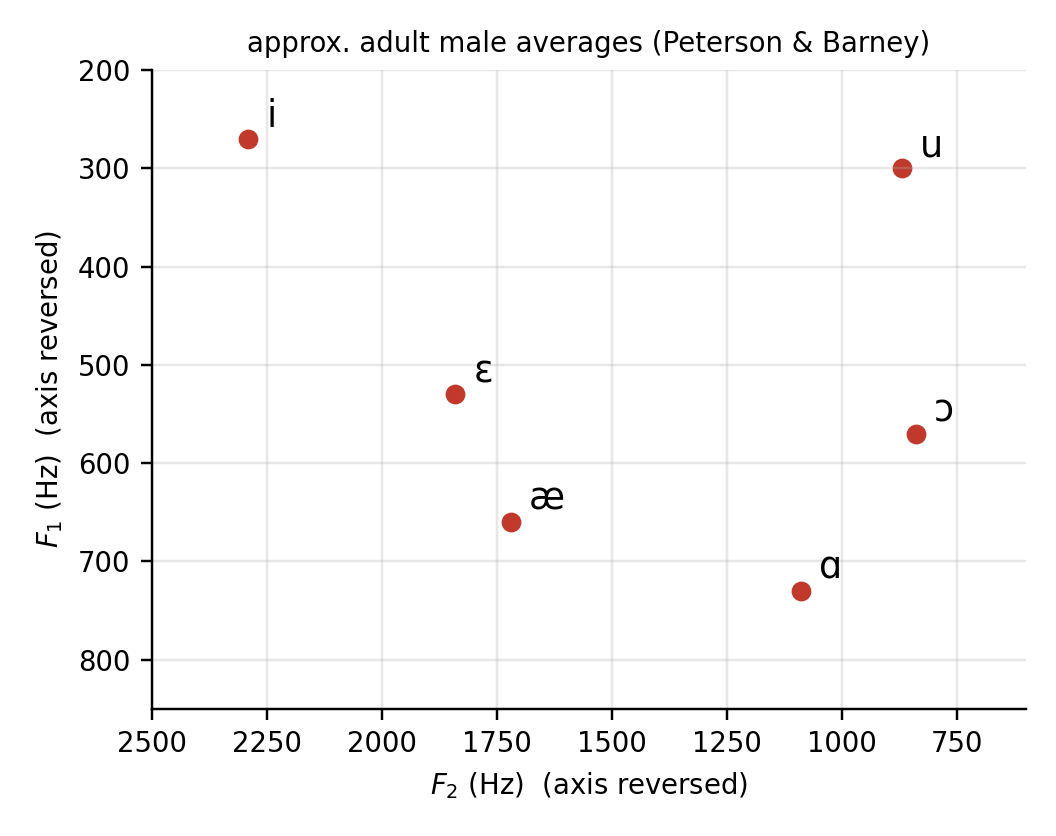
\includegraphics[width=0.55\textwidth]{../assets/figures/ch03-vowel-f1f2.png}
\caption{نقشهٔ آکوستیکی واکه‌ها در صفحهٔ $F_1$--$F_2$ (محورها معکوس)؛ شبیه نقشهٔ واکه‌ها در آواشناسی تولیدی (شکل افزوده).}
\end{figure}

\textbf{طول مجرا:} مجرای بلندتر، فرمنت‌ها را پایین‌تر می‌برد و مجرای کوتاه‌تر بالاتر (مجرای مردان معمولاً بلندتر است). این یکی از دلایلی است که $F_0$ به‌تنهایی جنسیت را مشخص نمی‌کند.

\begin{center}
\begin{tabular}{p{2.6cm}p{4.6cm}p{5.4cm}}
\toprule
ویژگی & هارمونیک & فرمنت \\
\midrule
منشأ اصلی & تناوب منبع (تارها) & تشدیدهای مجرای صوتی \\
نوع نمایش & مؤلفه در فرکانس مشخص & ناحیه یا قلهٔ تشدیدی در پوش طیف \\
ارتباط با $F_0$ & مضارب صحیح $F_0$ & لزوماً مضرب صحیح نیست \\
\bottomrule
\end{tabular}
\end{center}

\textbf{مثال کلاسی.} فرض کنید $F_0=120$ هرتز؛ هارمونیک‌ها $120,240,360,480,600,720,840,960,\dots$ هستند. اگر $F_1=750$ هرتز باشد، کدام هارمونیک‌ها بیشتر تقویت می‌شوند؟ پاسخ: ششم (۷۲۰) و هفتم (۸۴۰) که به ۷۵۰ نزدیک‌ترند (فاصله‌ها: $30$ و $90$ هرتز). میزان دقیق تقویت به شکل و پهنای قلهٔ تشدیدی بستگی دارد؛ به همین دلیل فرمنت در اسپکتروگرام یک ناحیهٔ پررنگ است، نه یک خط (شکل \ref{fig:ch03-harmonics-f1}).

\begin{figure}[htbp]
\centering
\begin{tikzpicture}[rtl, x=1cm,y=1cm,scale=1]
\def\u{0.0088}% cm per Hz
\fill[softblue] plot[smooth,domain=0:1340,samples=60] (\u*\x,{0.1+2.0*exp(-((\x-750)/230)^2)}) -- (\u*1340,0) -- (0,0) -- cycle;
\draw[mainblue, thick, smooth, domain=0:1340, samples=60, variable=\x] plot (\u*\x,{0.1+2.0*exp(-((\x-750)/230)^2)});
\foreach \n in {1,...,11}{
  \pgfmathtruncatemacro{\f}{120*\n}
  \pgfmathsetmacro{\h}{0.1+2.0*exp(-((\f-750)/230)^2)}
  \ifnum\n=6 \def\c{red!75!black}\def\w{1.8pt}\else\ifnum\n=7 \def\c{red!75!black}\def\w{1.8pt}\else\def\c{black!65}\def\w{0.9pt}\fi\fi
  \draw[\c, line width=\w] (\u*\f,0) -- (\u*\f,\h);
  \node[font=\scriptsize, below=1pt] at (\u*\f,0) {\lr{\n}};
  \node[font=\scriptsize, below=11pt, text=black!70] at (\u*\f,0) {\lr{\f}};
}
\draw[-{Stealth[length=2mm]}, thick] (0,0) -- (\u*1400,0) node[right, font=\small] {\lr{Hz}};
\draw[dashed, red!75!black] (\u*750,0) -- (\u*750,2.65);
\node[above, font=\small, red!75!black] at (\u*750,2.65) {\lr{$F_1=750$ Hz}};
\node[font=\scriptsize, anchor=east] at (-0.15,-0.2) {شماره};
\node[font=\scriptsize, anchor=east, text=black!70] at (-0.15,-0.62) {\lr{$nF_0$}};
\end{tikzpicture}
\caption{مثال تخته: با $F_0=120$ هرتز و $F_1=750$ هرتز، هارمونیک‌ها در ۱۲۰، ۲۴۰، ۳۶۰، \dots هرتز قرار دارند و شمارهٔ هرکدام زیر آن نوشته شده است. هارمونیک‌های نزدیک به قلهٔ تشدیدی (ششم و هفتم، ۷۲۰ و ۸۴۰ هرتز، با رنگ قرمز) بیشترین تقویت را می‌گیرند؛ منحنی آبی شکل کلی فیلتر مجرای صوتی است (منحنی افزوده) (بازسازی‌شده از تختهٔ کلاس).}
\label{fig:ch03-harmonics-f1}
\end{figure}

\section{اسپکتروگرام باند باریک و باند پهن}

کلید فهم این دو نوع، یک مبادله (\eng{trade-off}) بنیادی است: پنجرهٔ \textbf{کوتاه} تغییرات سریع زمانی را بهتر نشان می‌دهد ولی فرکانس‌های نزدیک را بد تفکیک می‌کند؛ پنجرهٔ \textbf{بلند} برعکس. وضوح فرکانسی تقریباً با معکوس طول پنجره متناسب است ($\Delta f\sim 1/L$؛ مثلاً با $f_s=16000$ و $N=512$ نمونه، $\Delta f=31.25$ هرتز).

\begin{definitionbox}{باند پهن در برابر باند باریک}
\textbf{باند پهن (\lr{Wideband}):} پنجرهٔ کوتاه (حدود ۳ تا ۵ میلی‌ثانیه؛ در کلاس ۵). وضوح زمانی بالا، وضوح فرکانسی پایین؛ هارمونیک‌ها در هم ادغام می‌شوند و پوش طیفی (فرمنت‌ها) دیده می‌شود.

\textbf{باند باریک (\lr{Narrowband}):} پنجرهٔ بلندتر (حدود ۲۰ تا ۵۰ میلی‌ثانیه؛ در کلاس ۳۰). وضوح فرکانسی بالا، وضوح زمانی پایین؛ هارمونیک‌ها به‌صورت خطوط افقی باریک و مجزا دیده می‌شوند.
\end{definitionbox}

\begin{center}
\begin{tabular}{lcc}
\toprule
ویژگی & باند پهن & باند باریک \\
\midrule
طول پنجره & کوتاه & بلند \\
وضوح زمانی & بالا & پایین \\
وضوح فرکانسی & پایین & بالا \\
نمایش مناسب‌تر & فرمنت‌ها & هارمونیک‌ها \\
\bottomrule
\end{tabular}
\end{center}

\begin{exambox}{نکتهٔ مهم استاد}
این دو نوع اسپکتروگرام مربوط به دو سیگنال متفاوت نیستند؛ هر دو از \emph{یک} سیگنال با تنظیم متفاوت پنجره ساخته می‌شوند. دقت زمانی و فرمنت $\Leftarrow$ \eng{wideband}؛ دقت فرکانسی و هارمونیک‌ها $\Leftarrow$ \eng{narrowband}.
\end{exambox}

فرمنت‌ها با حرکت سریع زبان و دهان تغییر می‌کنند و ردگیری آن‌ها وضوح زمانی خوب می‌خواهد؛ به همین دلیل باند پهن برای فرمنت‌ها مناسب‌تر است.

\begin{figure}[htbp]
\centering
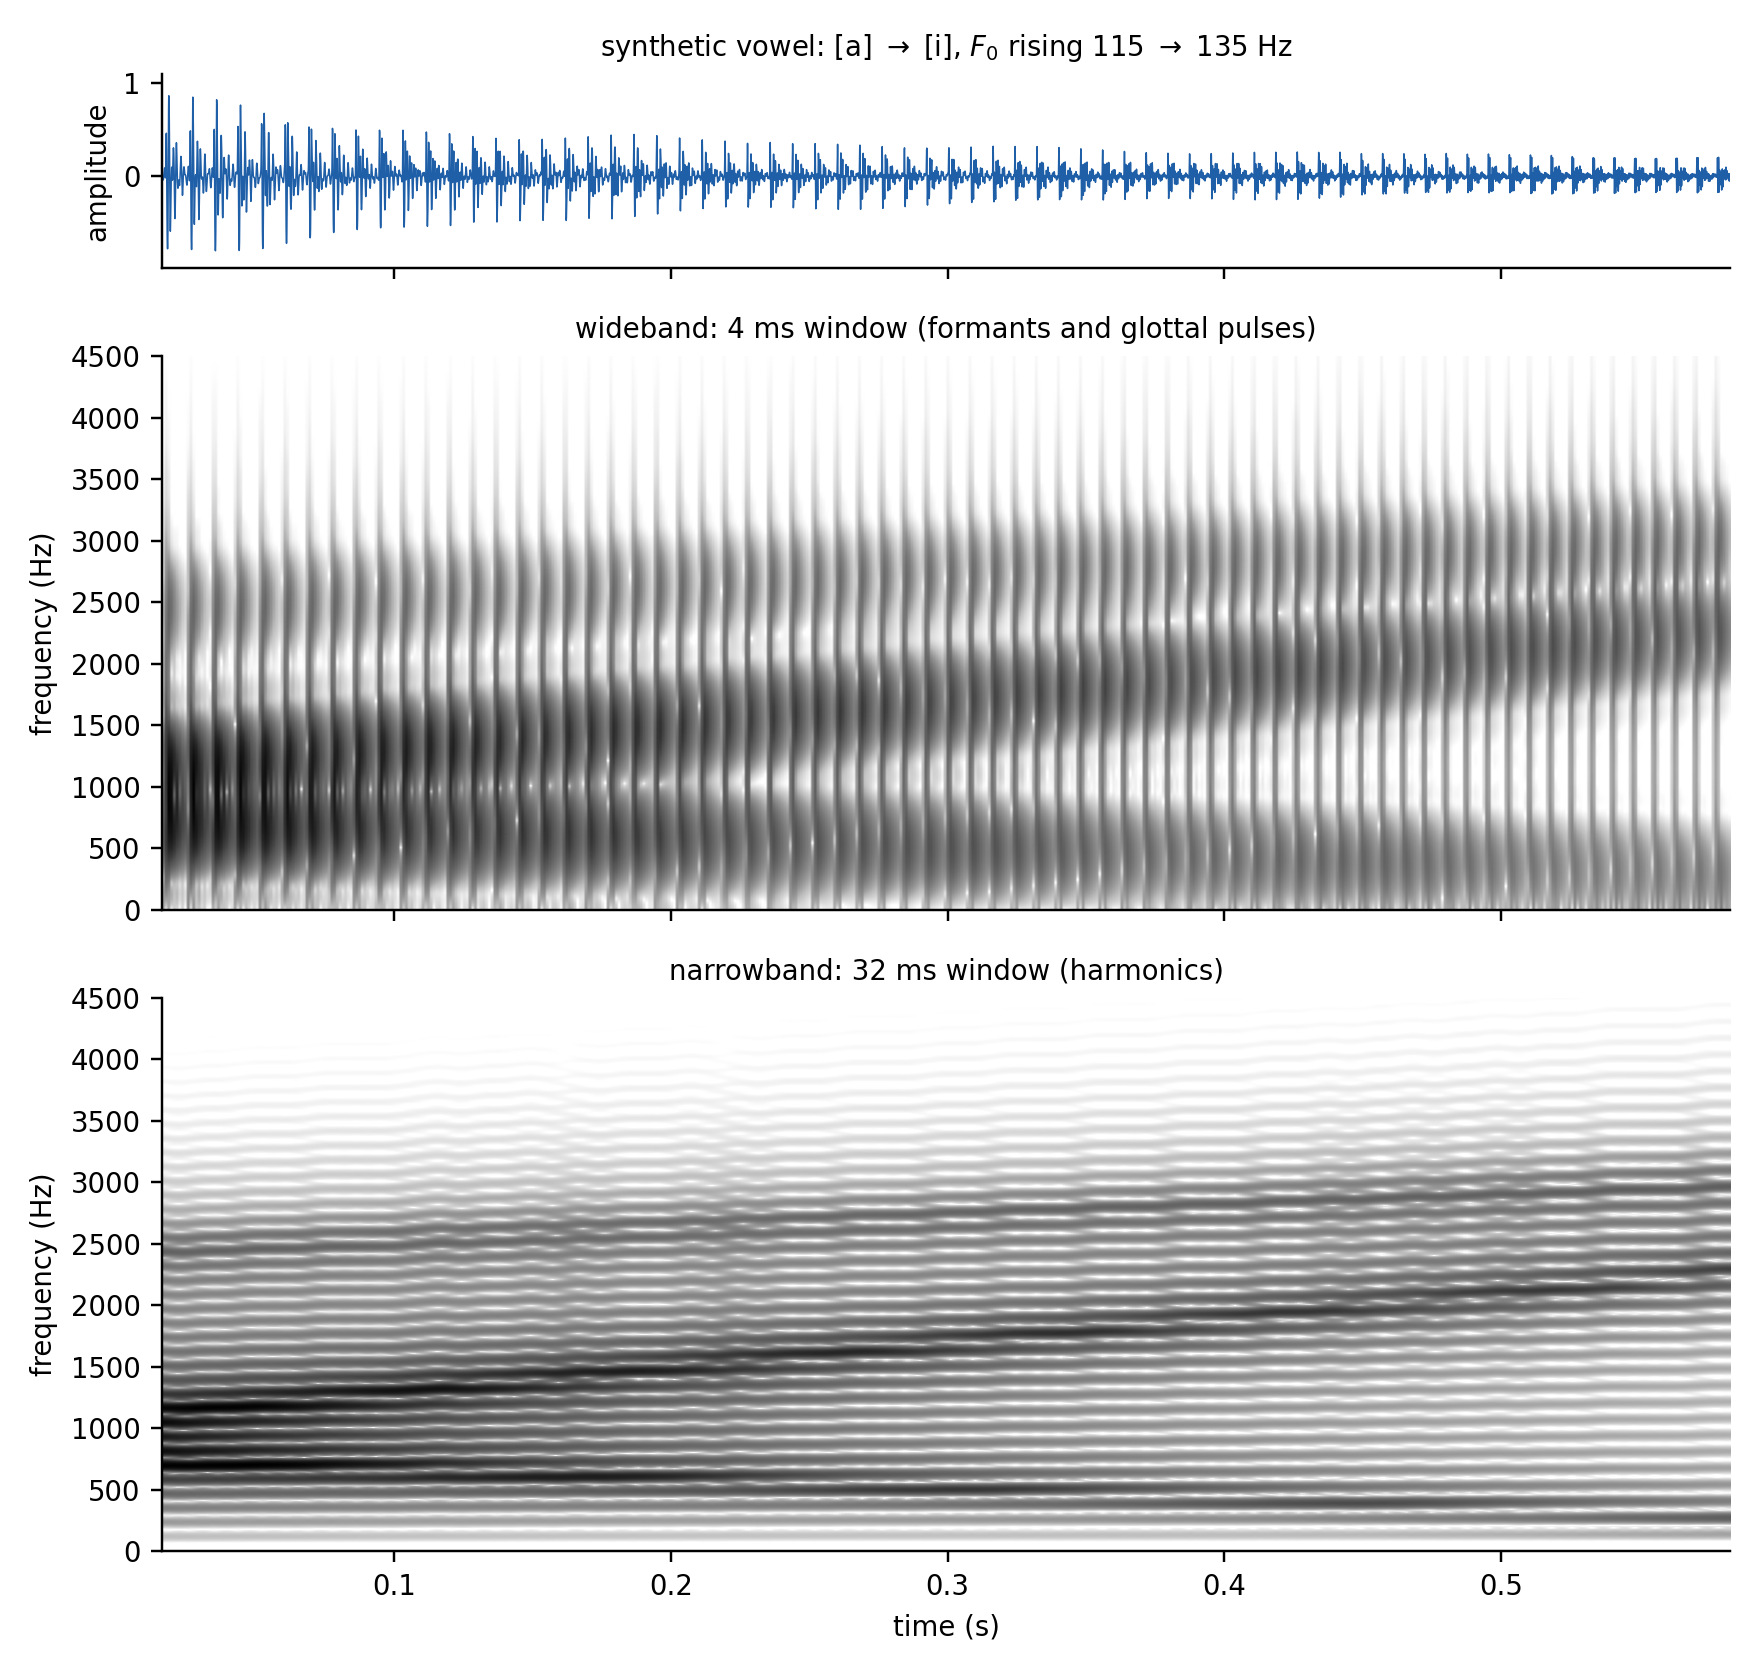
\includegraphics[width=0.95\textwidth]{../assets/figures/ch03-wideband-narrowband.png}
\caption{اسپکتروگرام باند پهن (پنجرهٔ ۴ میلی‌ثانیه) و باند باریک (۳۲ میلی‌ثانیه) از \emph{یک} واکهٔ ترکیبی که از «آ» به «ای» می‌رود. باند پهن نوارهای فرمنتی و خطوط عمودی تپ‌های چاکنایی را نشان می‌دهد؛ باند باریک خطوط افقی هارمونیک‌ها را (شکل افزوده).}
\end{figure}

\section{پرسش و پاسخ}

\begin{itemize}
  \item \textbf{آیا هارمونیک‌ها و فرمنت‌ها را می‌توان کاملاً جدا کرد؟} خیر؛ فیلتر روی طیف منبع اثر گذاشته و هر دو در سیگنال حضورند. با تغییر نوع اسپکتروگرام فقط یکی بهتر دیده می‌شود.
  \item \textbf{اگر دهان ثابت بماند، فرمنت‌ها حذف می‌شوند؟} خیر؛ فیلتر همچنان هست و فرمنت‌ها نوارهای افقی نسبتاً ثابت‌اند.
  \item \textbf{آیا با تغییر فرمنت‌ها \eng{Pitch} از بین می‌رود؟} خیر؛ فیلتر بر دامنهٔ هارمونیک‌ها اثر می‌گذارد، نه بر $F_0$.
  \item \textbf{آیا فرمنت‌ها را می‌توان عددی استخراج کرد؟} بله، به‌عنوان ویژگی عددی؛ الگوریتم‌هایش در این جلسه بررسی نشد.
\end{itemize}

\section{کاربردهای اسپکتروگرام و تمرین}

{\emergencystretch=3em اسپکتروگرام ابزاری آموزشی نیست و در مسائل واقعی مانند \term{تشخیص احساس از گفتار}{Speech Emotion Recognition} به کار می‌رود. در بخش عملی، استاد ابزاری پایتونی (مبتنی بر پردازش سیگنال، با کاربرد در گفتاردرمانی) را روی کلمهٔ «سیب» نشان دادند: در نمایش اول خطوط هارمونیکی واضح‌تر بودند و برای دیدن بهتر فرمنت‌ها باید اندازهٔ پنجره را کوتاه کرد (باند پهن).\par}

\begin{assignmentbox}{تمرین اول: اسپکتروگرام}
تمرین اول با اسپکتروگرام مرتبط است؛ جزئیات اجرایی در این جلسه بیان نشد. مفاهیم لازم: شکل موج، $F_0$ و هارمونیک‌ها، تبدیل فوریه و پنجره‌بندی، تولید و تحلیل اسپکتروگرام، تفاوت باند پهن و باریک، و مشاهده و تفسیر فرمنت‌ها.
\end{assignmentbox}

\section{جمع‌بندی}

\begin{center}
\begin{tabular}{p{3.4cm}p{9.4cm}}
\toprule
مفهوم & تعریف و نقش \\
\midrule
فرکانس پایه $F_0$ & $1/T_0$؛ مرتبط با \eng{Pitch}؛ وابسته به طول، جرم و کشش تارها \\
هارمونیک‌ها & مضارب صحیح $F_0$، با فاصلهٔ $F_0$ \\
اسپکتروگرام & بزرگی \eng{STFT}؛ محتوای فرکانسی در طول زمان \\
منبع / فیلتر & تارهای صوتی (واک‌دار) / مجرای صوتی که طیف منبع را شکل می‌دهد \\
فرمنت‌ها & نواحی تشدید مجرا ($F_1<F_2<F_3$)؛ $F_1$: ارتفاع/بازشدگی، $F_2$: جلو--عقب \\
باند پهن / باریک & پنجرهٔ کوتاه، فرمنت‌ها / پنجرهٔ بلند، هارمونیک‌ها \\
\bottomrule
\end{tabular}
\end{center}

رابطه با جلسهٔ قبل: آواشناسی تولیدی وضعیت اندام‌ها را توصیف می‌کند؛ مدل منبع--فیلتر آن را به تحریک تارها و فیلتر مجرا ترجمه می‌کند؛ $F_0$، هارمونیک‌ها و فرمنت‌ها آثار قابل‌اندازه‌گیری آن هستند و اسپکتروگرام ابزار مشاهدهٔ آن‌ها است.

\begin{exambox}{نکات مهم برای مرور و امتحان}
\begin{itemize}
  \item نمره: ۱۰ عملی (گزارش یا ارائه) + ۱۰ نظری (میان‌ترم و پایان‌ترم)؛ تمرین اول دربارهٔ اسپکتروگرام است.
  \item $F_0$ ویژگی فیزیکی و \eng{Pitch} ادراکی است؛ $F_0$ بالاتر یعنی صدای زیرتر. $F_0$ به‌تنهایی جنسیت را تعیین نمی‌کند؛ طول مجرا نیز مؤثر است.
  \item هارمونیک‌ها در $nF_0$ و با فاصلهٔ $F_0$ هستند؛ $F_0$ بزرگ‌تر یعنی هارمونیک‌های دورتر.
  \item اسپکتروگرام = پنجره‌بندی + فوریه برای هر پنجره + کنار هم چیدن (افقی زمان، عمودی فرکانس، رنگ بزرگی). فرکانس و دامنه متفاوت‌اند.
  \item $\text{Output}(f)=\text{Source}(f)\times\text{Filter}(f)$؛ منبع = تارها (واک‌دار)، فیلتر = مجرا.
  \item فرمنت ناحیهٔ تشدیدی مجراست، نه یک هارمونیک؛ $F_1$ با ارتفاع/بازشدگی و $F_2$ با جلو/عقب بودن زبان مرتبط است؛ مجرای بلندتر، فرمنت‌های پایین‌تر. فرمنت‌ها «شناسایی» می‌شوند، نه «ساخته».
  \item باند پهن (پنجرهٔ حدود ۵ میلی‌ثانیه) $\leftarrow$ فرمنت‌ها و وضوح زمانی؛ باند باریک (حدود ۳۰ میلی‌ثانیه) $\leftarrow$ هارمونیک‌ها و وضوح فرکانسی؛ هر دو از یک سیگنال‌اند.
  \item مثال کلاسی: $F_0=120$ و $F_1=750$ هرتز $\Leftarrow$ هارمونیک‌های ششم (۷۲۰) و هفتم (۸۴۰) بیشتر تقویت می‌شوند.
\end{itemize}
\end{exambox}
